\documentclass[]{scrartcl}
\usepackage{Preamble}

\renewcommand{\exercise}{Exercise 2}
\renewcommand{\duedate}{2020-06-08, 18:00}

\begin{document}
\section{Buffer}
\subsection{Auslastung von line}
\begin{figure}[ht]
    \centering
    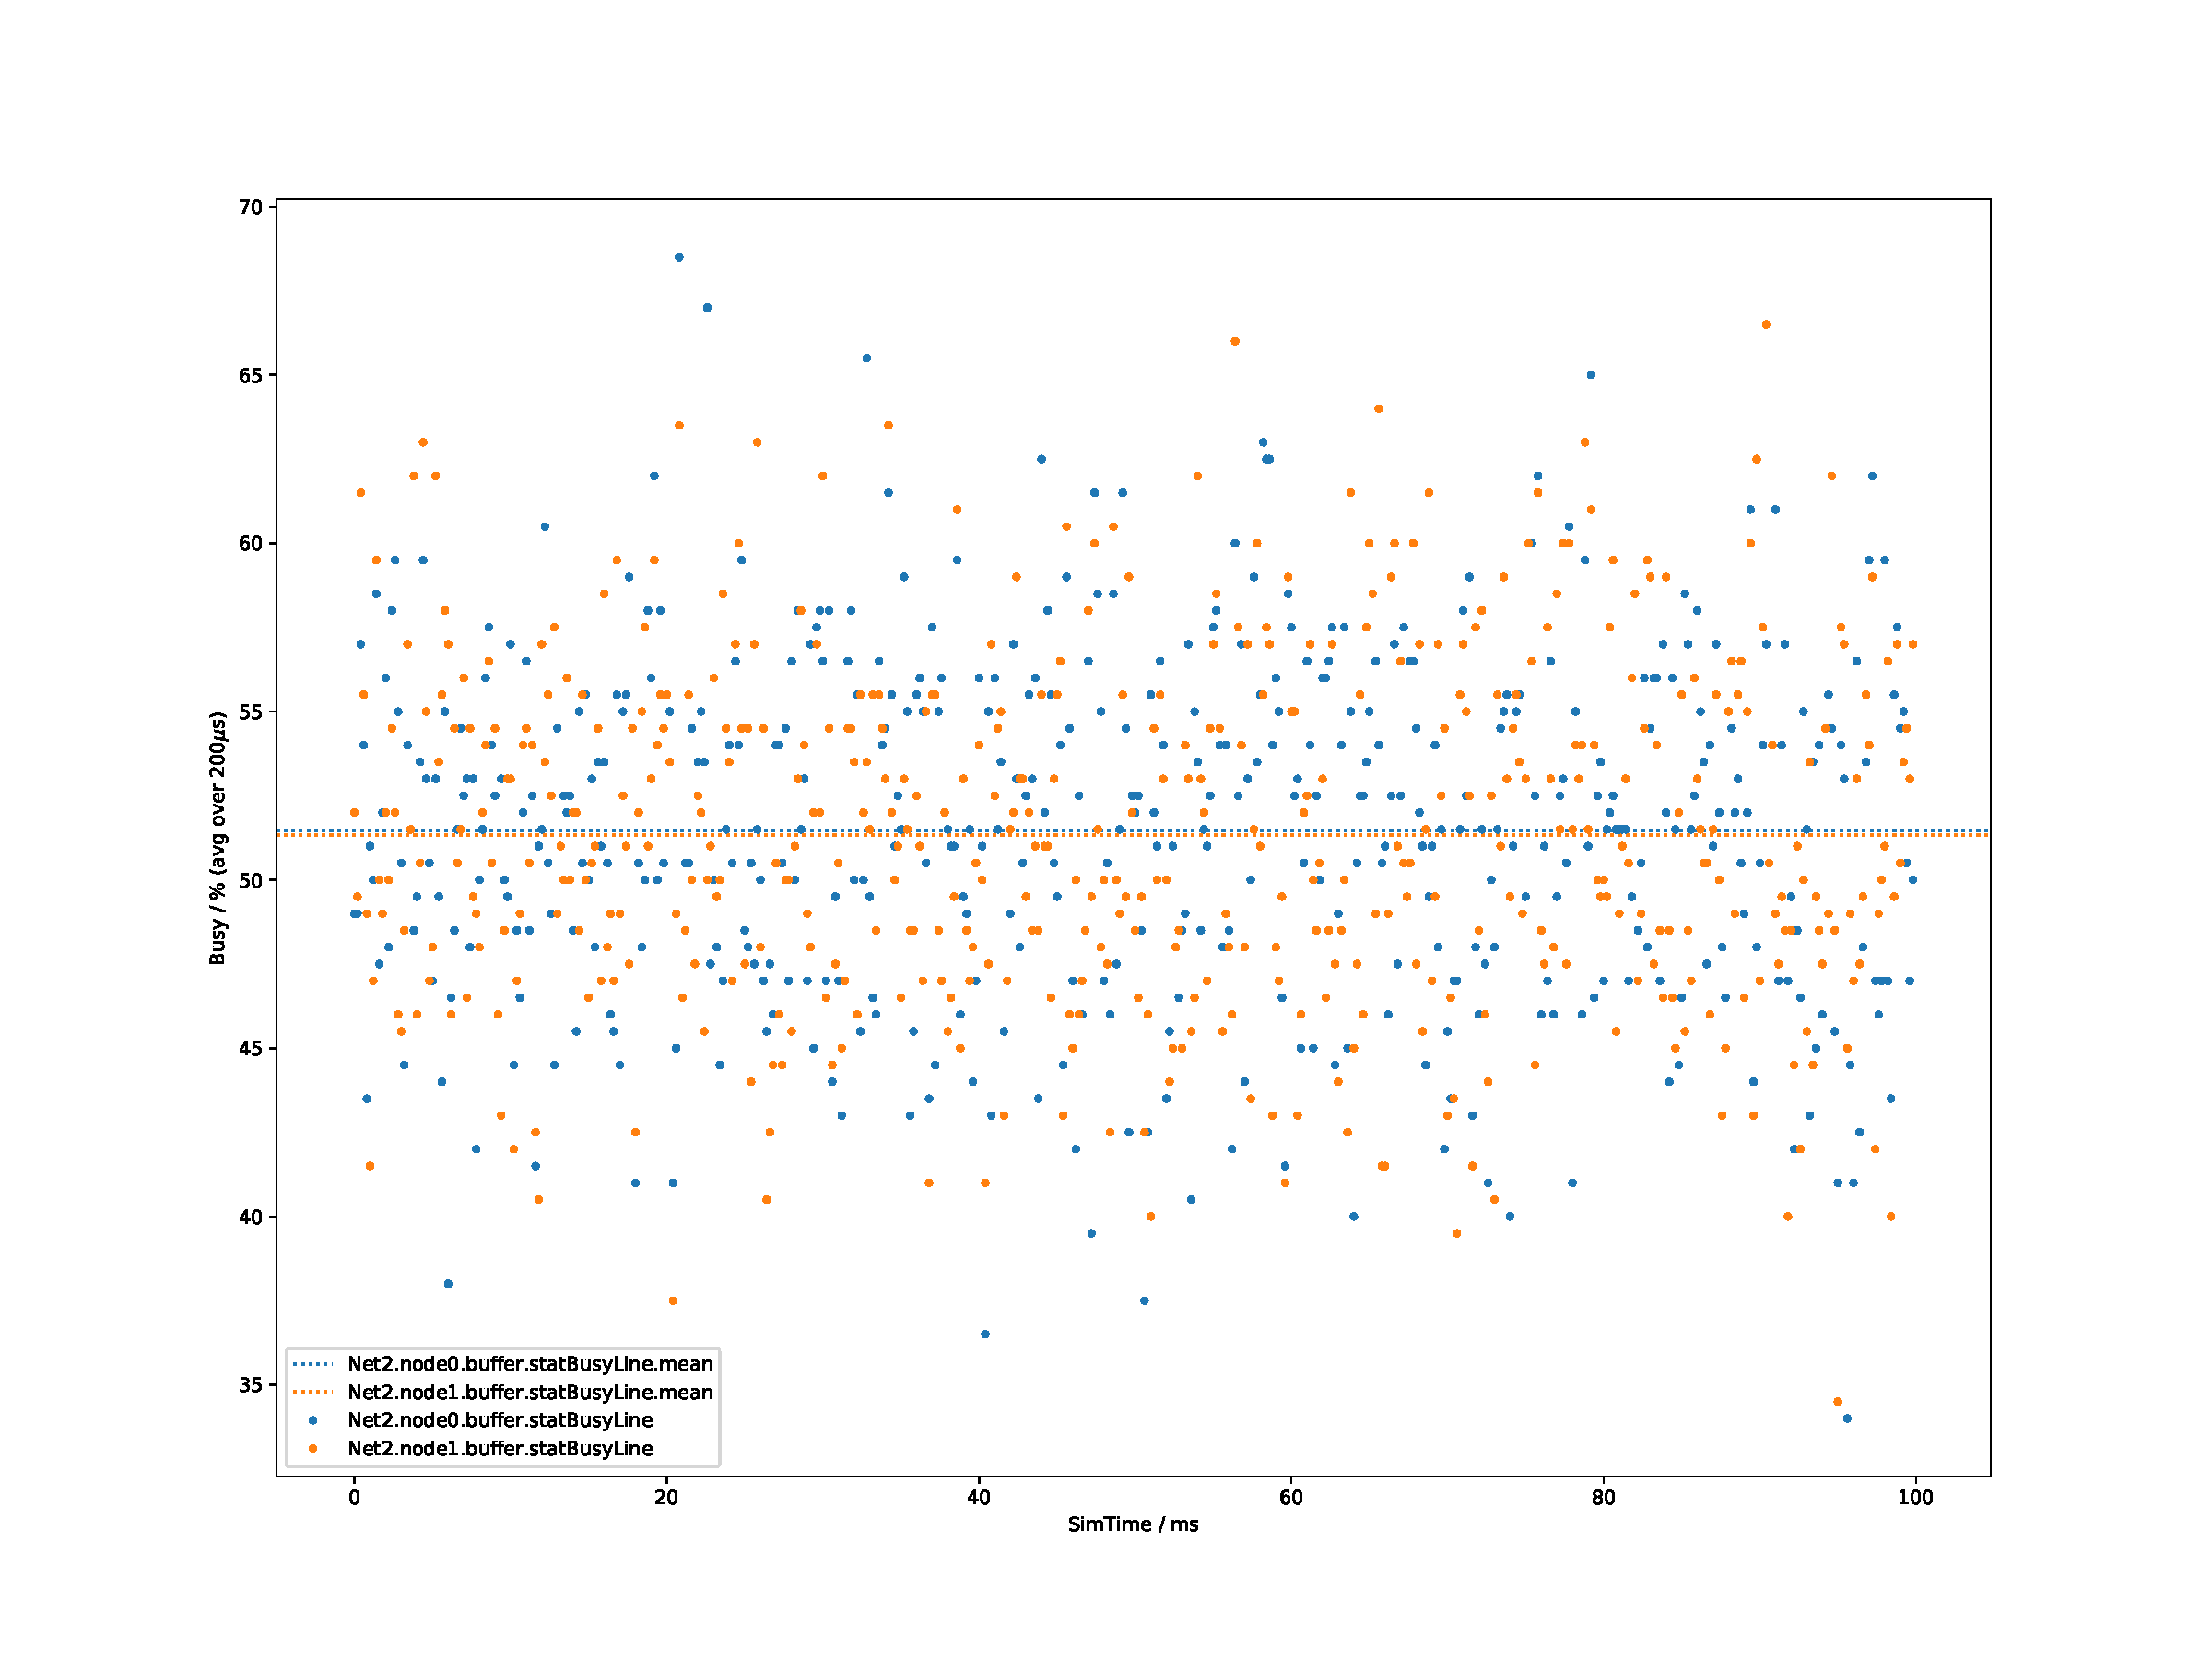
\includegraphics[width=\columnwidth]{../../python/03_01.pdf}
    \caption{Auslastung von line, bei einer Abfragefrequenz von \SI{1}{GHz} und der Mittelung von 200 Abfragen}
\end{figure}
\newpage
\subsection{Number of Packets waiting in Queue}
\begin{figure}[ht]
    \centering
    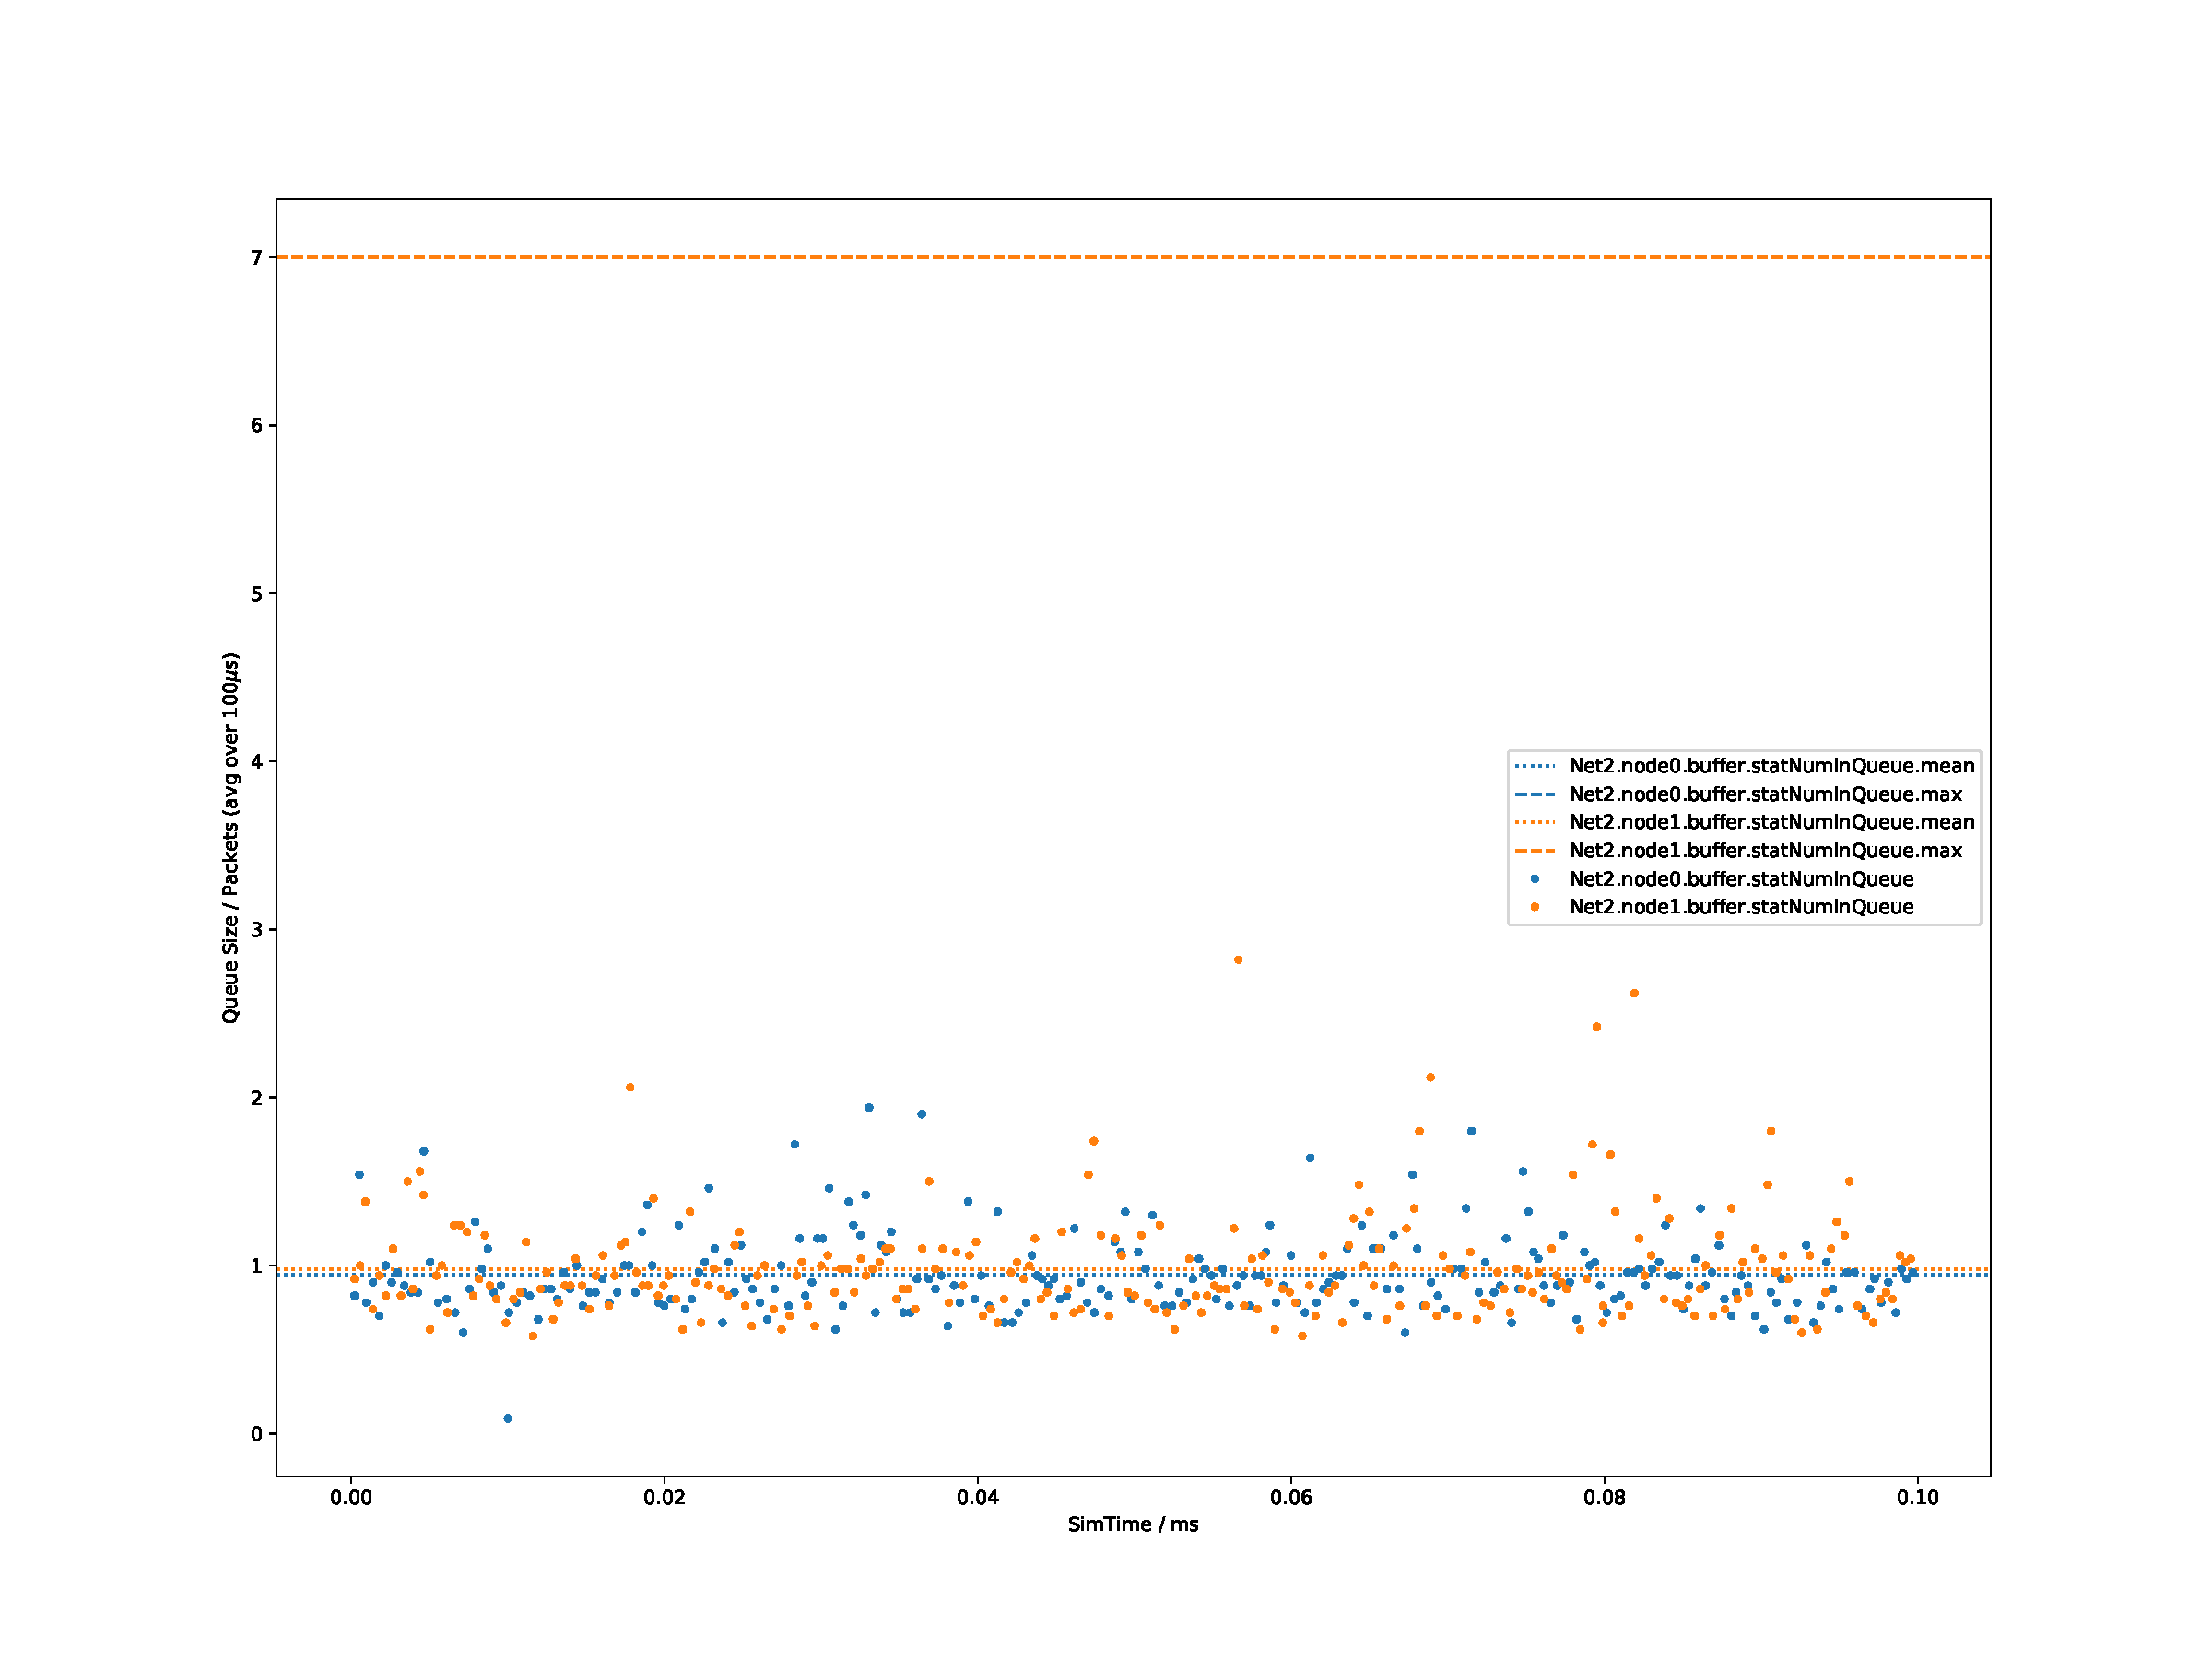
\includegraphics[width=\columnwidth]{../../python/03_02.pdf}
    \caption{}
\end{figure}
\end{document}
